\documentclass[11pt]{article}
%============= Imports =============
\usepackage{physics}
\usepackage{amsmath,amsthm,amssymb}
\usepackage[dvips,letterpaper,margin=0.9in,bottom=0.7in]{geometry}
\usepackage{hyperref}
\usepackage{enumitem}
\usepackage{charter}
\usepackage{tabstackengine}
\usepackage{fancyhdr}
\usepackage{graphicx}
\usepackage{subfig}
\usepackage{siunitx}
\usepackage{float}
\usepackage{listings}
\usepackage{xcolor}
\usepackage{natbib}
\bibliographystyle{apa-good}
%============= Page style =============
\pagestyle{fancy}
\newcommand{\CourseDef}{PHY424} %Course
\newcommand{\TitleDef}{Statistics of trefoil knot opening times in vibrated granular chains} %Title
\newcommand{\NumberDef}{1006154625}
\newcommand{\AuthorDef}{Lucas Prates} %Author (Name)
\rhead{\AuthorDef}
\chead{\TitleDef}
\lhead{\CourseDef}
\definecolor{codegreen}{rgb}{0,0.6,0}
\definecolor{codegray}{rgb}{0.5,0.5,0.5}
\definecolor{codepurple}{rgb}{0.58,0,0.82}
\definecolor{backcolour}{rgb}{0.95,0.95,0.92}
\lstdefinestyle{mystyle}{
    backgroundcolor=\color{backcolour},   
    commentstyle=\color{codegreen},
    keywordstyle=\color{magenta},
    numberstyle=\tiny\color{codegray},
    stringstyle=\color{codepurple},
    basicstyle=\ttfamily\footnotesize,
    breakatwhitespace=false,         
    breaklines=true,                 
    captionpos=b,                    
    keepspaces=true,                 
    numbers=left,                    
    numbersep=5pt,                  
    showspaces=false,                
    showstringspaces=false,
    showtabs=false,                  
    tabsize=2
}

\lstset{style=mystyle}
%============= Matrix Commands =============
\setstackEOL{;}% row separator
\setstackTAB{,}% column separator
\setstacktabbedgap{2ex}% inter-column gap
\setstackgap{L}{1.0\normalbaselineskip}% inter-row baselineskip
\let\bmatrix\bracketMatrixstack
\let\pmatrix\parenMatrixstack
\let\dmatrix\vertMatrixstack
\newcommand{\declarecommand}[1]{\providecommand{#1}{}\renewcommand{#1}}
%============= Other Commands =============
\declarecommand{\R}{\mathbb{R}}
\declarecommand{\Q}{\mathbb{Q}}
\declarecommand{\Z}{\mathbb{Z}}
\declarecommand{\N}{\mathbb{N}}
\declarecommand{\C}{\mathbb{C}}
\declarecommand{\emptyset}{\varnothing}
\newcommand{\mat}[1]{\begin{bmatrix}#1\end{bmatrix}}
%%[label=(alph*)]
%============= Title Config =============
%\title{\CourseDef\space\TitleDef}
%\author{\AuthorDef \\ \NumberDef}
\begin{document}
\thispagestyle{plain}
{\noindent\Huge\bf  \\[0.5\baselineskip] {\fontfamily{cmr}\selectfont  \TitleDef}         }\\[2\baselineskip] % Title
{ {\bf \fontfamily{cmr}\selectfont \CourseDef}\\ {\textit{\fontfamily{cmr}\selectfont     \today}}}\hspace{150pt}    {\large \textsc{\AuthorDef}} % Author name
\\[1.4\baselineskip]
\vspace{-15pt}

%\begin{figure}[h]%
%    \centering
%    \subfloat{{\includegraphics[scale=0.56]{Kp_Upstream_figure.png} }}%
%    \qquad
%    \subfloat{{\includegraphics[scale=0.56]{Kp_Downstream_figure.png} }}%
%    \caption{Time-averaged $K_{\rho}^U$ (a) and $K_{\rho}^D$ (b) for each simulation. The time average was taken        on the last $54t_0$ ($\sim20$ minutes of simulation time) of the simulation.}%
%    \label{fig:diffus}%
%\end{figure}
%============= Start File =============

\begin{abstract}
    This paper details my study of the opening times of trefoil knots in vertically vibrated
    granular chains. I find strong evidence of a quadradic relationship between the trefoil's 
    mean opening time, $\tau_{\text{avg}}$, and the length of the granular chain, $N$. 
    Additionally, I find quantitative evidence that the knot's survival time distribution 
    $S(t,N)$ can be expressed as a function of a single parameter, $t/\tau_{avg}$.
\end{abstract}

\section{Introduction}
The thermal motion of filamentary objects such as DNA
and polymer micromolecules can often lead to the formation and opening of knots. 
Understanding these processes can lead to an understanding of the macroscopic properties 
of materials like gels and plastics \citep{Meluzzi2010}. In particular, understanding how 
topological constraints such as knots affect the dynamics of these one dimensional filaments 
is crucial in understanding the flow and structural properties of the materials they componse. 
Unfortunately, such constraints are diffucult to observe and manipulate at such a scale 
\citep{BenNaim2001}.\\

Using a macroscopic analogy for such a system is a good first step towards 
understanding the dynamics of knots in one dimensional filaments, at a scale where the knots can 
be easily manipulated and observed. In this experiment, I create a simple analog
by studying the dynamics of the trefoil knot in vertically vibrated ball chains.\\

In this paper, I seek to find a relationship between the chain length in number of balls, $N$, and 
the mean trefoil opening time, $\tau_{\text{avg}}$. Additionally, I study the survival probability
$S(t,N)$, which is the probability that a knot in a length $N$ chain still exists at time $t$. This paper 
seeks to show that $S(t,N)$ can be expressed as a function of a single variable, $z=t/\tau_{\text{avg}}$.
% \cite{BenNaim2001} models the average opening time of a 
% vertically vibrated trefoil knot in a ball chain of length $N$, where length is measured in 
% number of balls on the chain, as 
%     \begin{equation}
%         \label{eq:model}
%         \tau_{\text{avg}} \propto (N- N_0)^2
%     \end{equation}
% where $N_0$ is minimal size of the knot. That is, $N_0$ is the number of balls contained 
% in the knot when it has been pulled as tightly as possible.\\

% The survival probability of a knot in a chain of length $N$, denoted $S(t,N)$,
% is the probability that the knot has not yet opened at time $t$.
% \cite{BenNaim2001} postulates that $S(t,N)$ is a function of a single vairable. In particular, for
% the variable $z= t/ \tau_{\text{avg}}(N)$, 
%     \begin{equation}
%         \label{eq:survival}
%         S(t, N) = F(z)
%     \end{equation}

% In this paper, I seek to verify equations \ref{eq:model} and \ref{eq:survival}.

\section{Theory}
\label{sec:theory}
\cite{BenNaim2001} models the motion of a trefoil knot with minimum size $N_0$ as the random walk of three
independent point particles point particles which are not allowed to swap positions, along a one dimensional domain 
of size $N-N_0$, and identical diffusivity $D$. This essentially reduces to a three dimensional diffusion 
problem. By solving this diffusion problem with the appropriate assumptions, and intepreting 
the survival probability as the probability that the random walks remain confined to a finite 
domain, \cite{BenNaim2001} arrives at 
    \begin{equation}
        \label{eq:survival}
        S(t, N)= \Bigg( \frac{4}{\pi} \sum_{k=0}^{\infty} 
    \frac{\text{sin}[(2k+1)\pi x_0]}{2k+1} e^{-(2k+1)^2\pi^2 D t / (N - N_0)^2} \Bigg)^3
    \end{equation} 
where $x_0$ is the knot's initial fractional position along the chain.\\

Now, let $R(t, N)$ be the exit time distribution for the chain. Then, $R(t, N)dt$ can be
interpreted as the proportion of knots which open between $t$ and $t+dt$. The 
survival probability is the proportion of knots that remain unopened at time $t$. Then, 
    \begin{equation}
        \label{eq:exit-times}
        S(t, N) = 1 - \int_{0}^{t}R(\tilde{t}, N) d\tilde{t} \implies R(t, N) = -\derivative{S(t, N)}{t}
    \end{equation}
With this interpretation of the exit time distribution, the mean exit time can also be computed
using
\begin{equation}
    \label{eq:mean-exit-integral}
    \tau_{\text{avg}} = \int_{0}^{\infty} t R(t, N) dt
\end{equation}

Together with equations \ref{eq:survival} and \ref{eq:exit-times}, \ref{eq:mean-exit-integral} becomes

\begin{equation}
    \label{eq:mean-exit}
    \tau_{\text{avg}} = \frac{\tau_3}{D}(N-N_0)^2
\end{equation}
where $\tau_3 = 0.056213$. Thus, this equation gives the relationship between 
$\tau_{\text{avg}}$ and $N$ which I seek to verify. Finally, the function $F(z)$ may be defined as 
\begin{equation}
    \label{eq:characteristic}
    F(z) = \Bigg( \frac{4}{\pi} \sum_{k=0}^{\infty} 
    \frac{\text{sin}[(2k+1)\pi x_0]}{2k+1} e^{-(2k+1)^2\pi^2\tau_3 z} \Bigg)^3
\end{equation}
For $z=t/\tau_{\text{avg}}$, the survival probability can be expressed as $S(t, N) = F(z)$

\section{Experimental techniques}
\subsection{Materials}
    In this experiment I studied the behaviour of 1mm diameter yellow brass ball chains.
    I cut the chains to the desired length $N$ using a set of pliers, and tied a trefoil
    knot in its center (note that this corresponds to $x_0=1/2$ in equation \ref{eq:survival}). 
    For this to be easily repeatable, the center beads of 
    each chain were marked with black sharpie. For the yellow brass ball chains used in
    this experiment, $N_0=16$. Figure \ref{fig:chain} displays an example of a prepared chain.\\
    \begin{figure}[H]
        \centering
        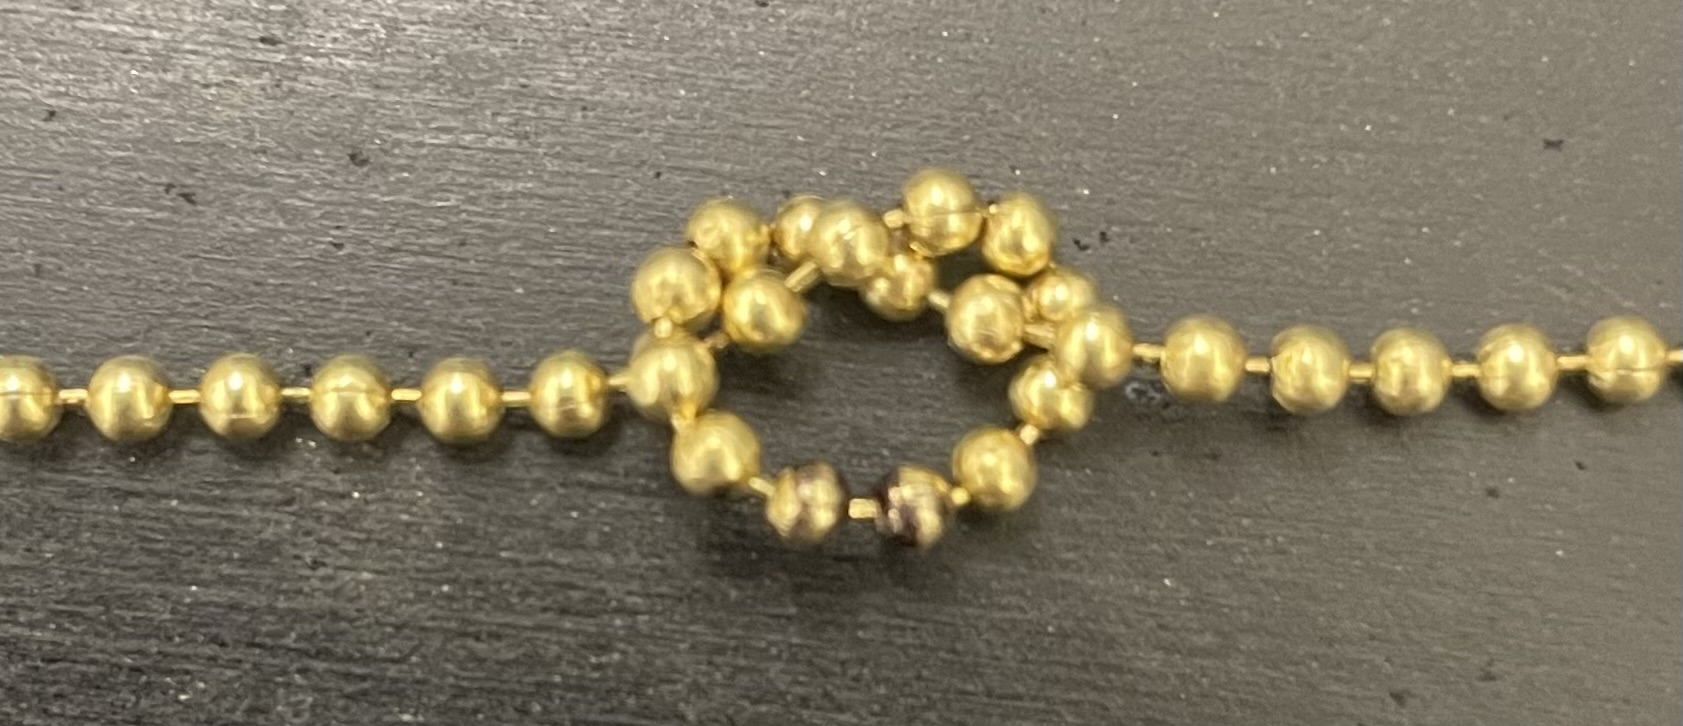
\includegraphics[scale=0.15]{chain.jpg}
        \caption{A trefoil knot in the yellow brass chain. The knot is tied to its minimum
        size, with $N_0=16$ interior beads. The center of the 
        chain is marked in black sharpie. Note the assymetry of the trefoil: the left arm 
        passes under the loop while the right arm passes over.}
        \label{fig:chain}
    \end{figure}
    The trefoil knot has a fundamental assymetry. One end of the knot must pass under the
    loop while the other passes over. To easily distinguish which end was which, I also 
    marked the end which was to pass over the loop in black sharpie.\\
    \begin{figure}[H]
        \centering
        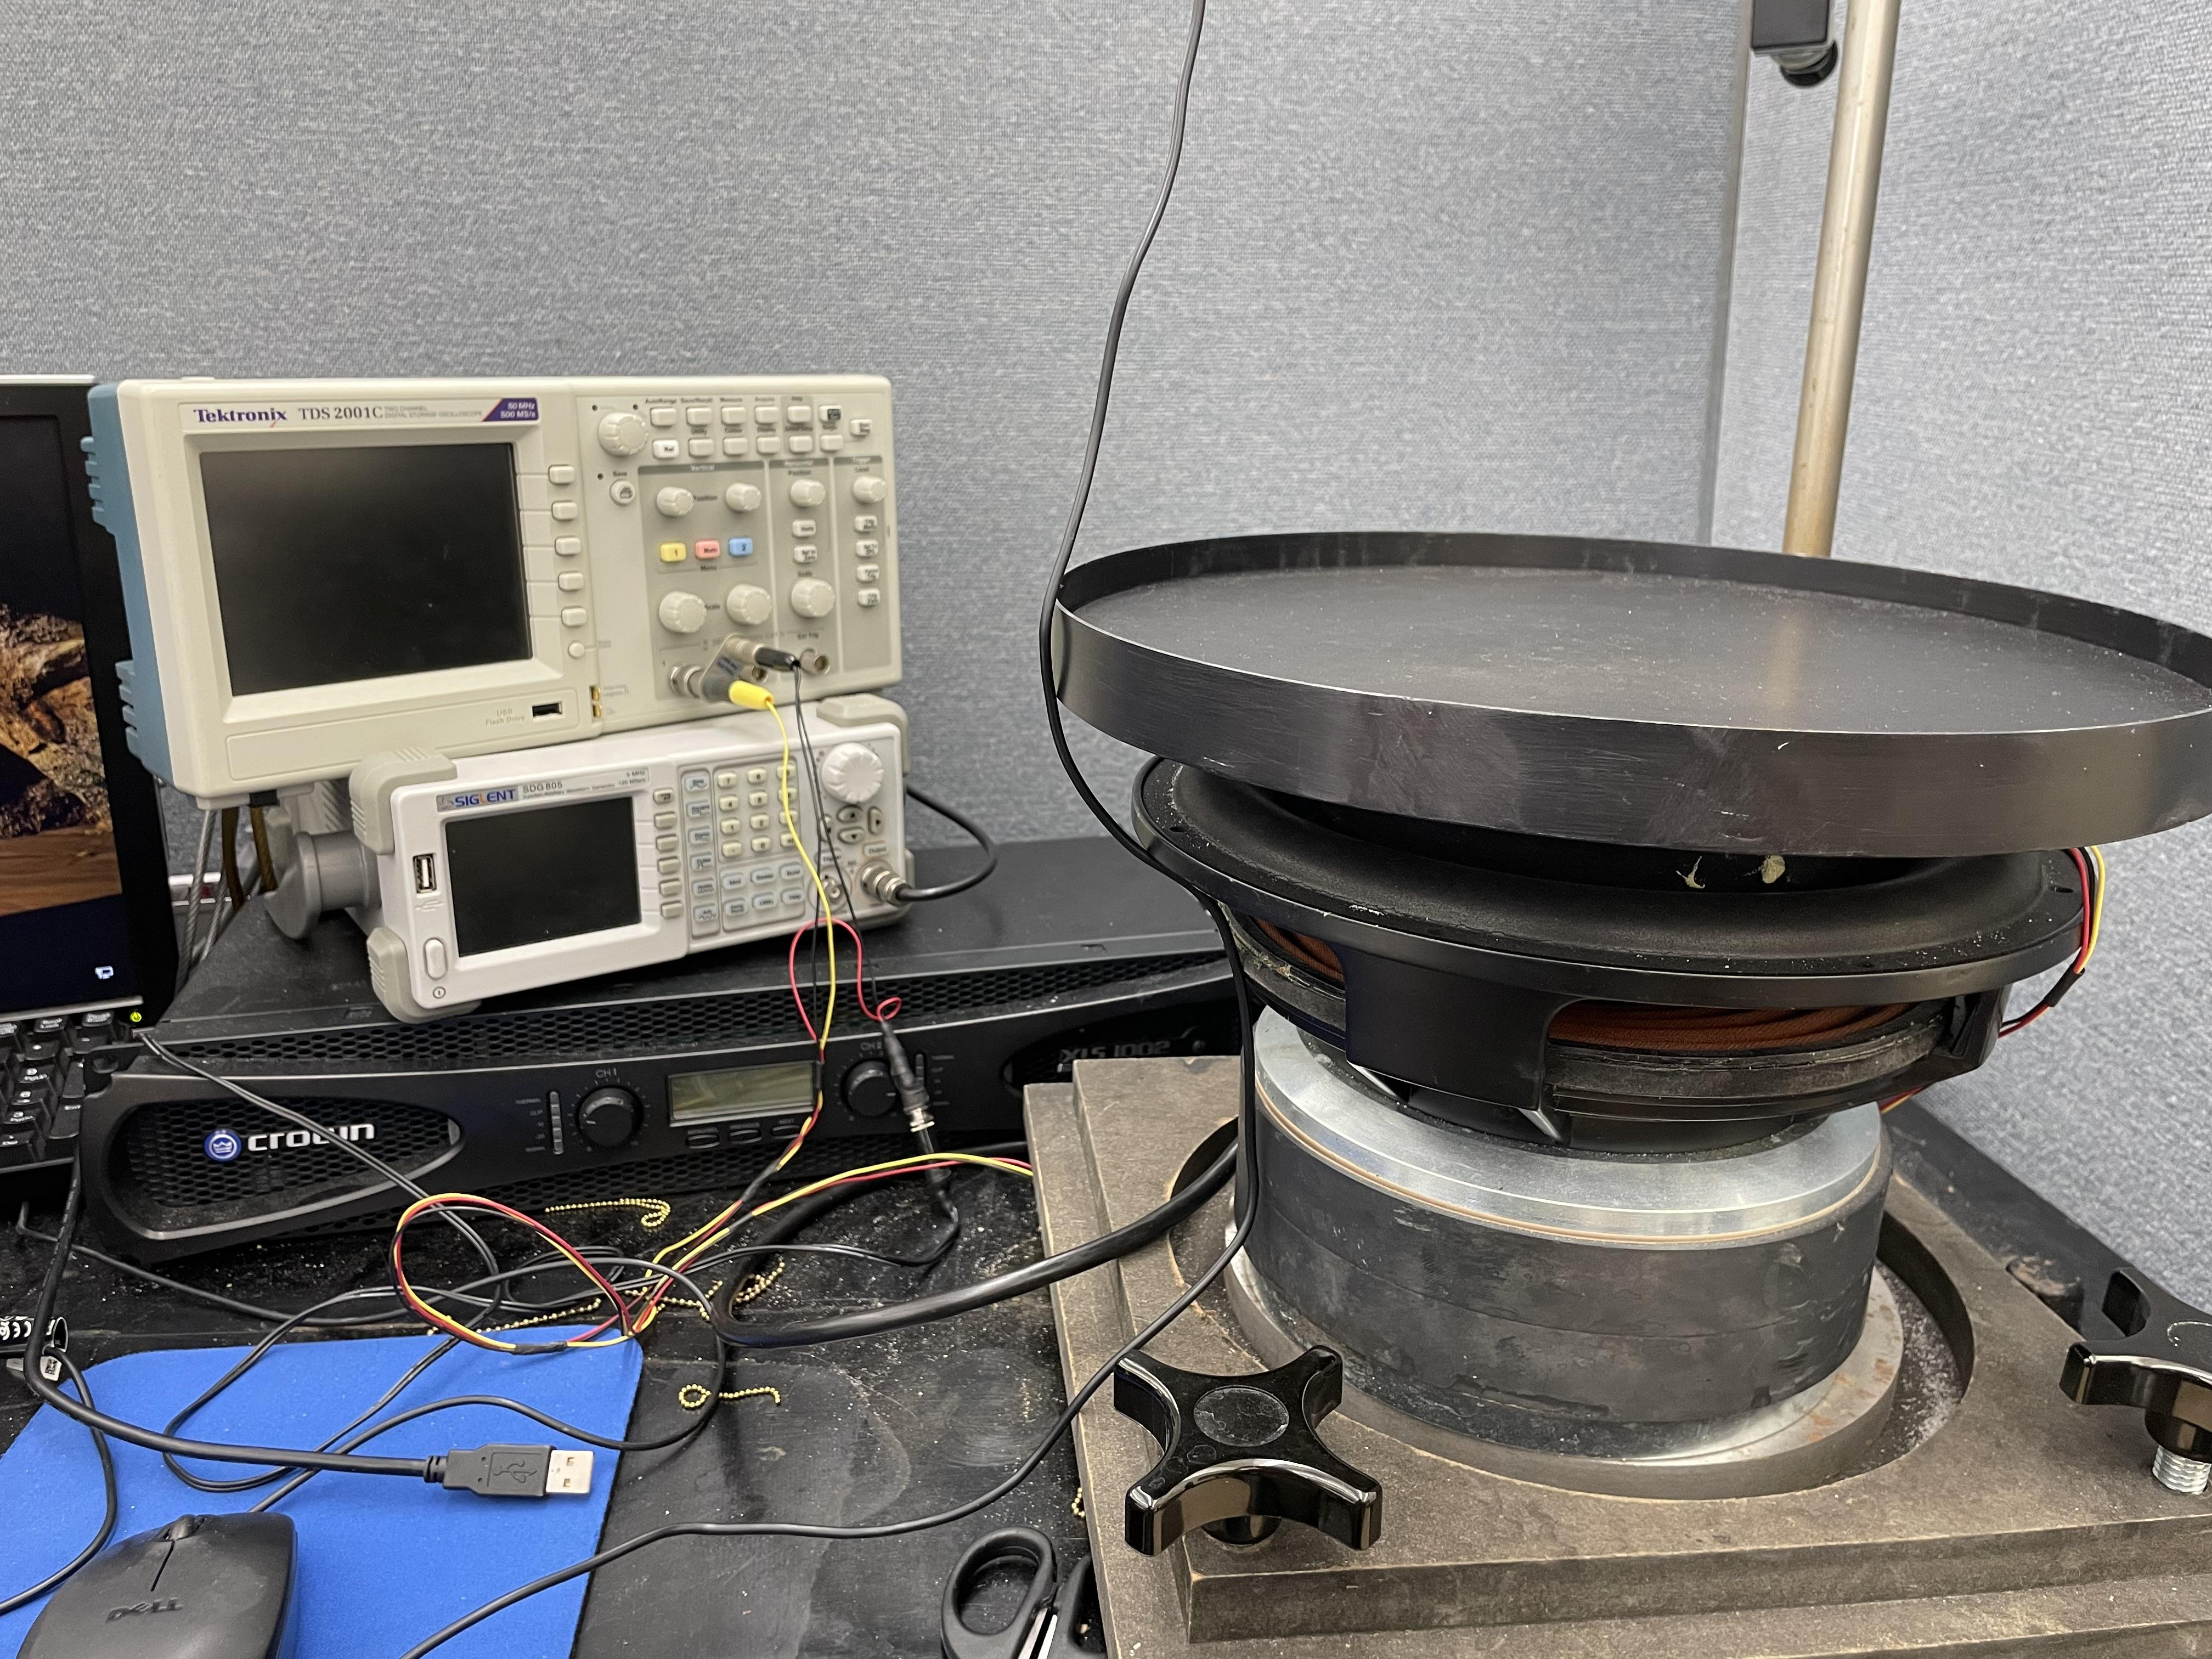
\includegraphics[scale=0.06]{setup.jpg}
        \caption{Pictured here is the alluminum shaker plate atop a speaker, driven by the power
        amplifier and signal generator. Atop the signal generator is the oscilloscope which reads the 
        accelerometer volatge outputs. The accelerometer is located under the shaker plate.}
        \label{fig:setup}
    \end{figure}
    The experimental apparatus, pictured in Figure \ref{fig:setup} consisted of an alluminum plate attatched to a magnetically 
    driven speaker, whose oscillations were determined by a signal generator. Attatched to
    the shaker plate was an accelerometer which sent a voltage proportional to shaker plate's acceleration
    to an oscilloscope. Since the shaker plate was driven sinusoidally, the 
    accelerometer voltage reading was also proportional to the amplitude of the plate's motion. Thus, 
    the oscilloscope voltage reading could be used as a measure of the plate amplitude.\\

\subsection{Methods}
    For this experiment, it was critical that the chain's motion was random, but not so intense 
    that the knot was allowed to flip or the chain to self-intersect, because such behaviours 
    violate Ben-Naim's assumptions outlined in Section \ref{sec:theory}. I found that driving the plate at a frequency of $f=13$Hz and 
    peak to peak amplitude of $A=840$mV worked well to satisfy these conditions. Although knot flipping 
    and self-intersection was not completely eliminated, these parameters caused it to happen infrequently 
    and also allowed for clear random motion of the chain. Additionally, any trials which saw 
    the knot drift into the wall of the alluminum plate were discarded.\\

    After preparing a length $N$ chain, I placed it on the center of the plate. For each trial, 
    I started the signal generator and began a timer. I stopped the timer when the knot opened (that is, 
    when one of the knot's arms passed through the loop). I then collected the final 
    time. Since there was a lag of about 1 second between the knot opening and my stopping the
    stopwatch, I tended to overestimate the opening times. This caused a systematic bias which was
    accounted for in the analysis phase.\\

    For each length of chain, I collected data until $d\tau_{\text{avg}}/\tau_{\text{avg}} \sim 0.1$, 
    where $d\tau_{\text{avg}}$ is the standard error in the mean. This usually took about 30-60 datapoints. I took $40 \leq N \leq 140$ with increments of 
    $20$. The lower bound was chosen based on the fact that $N_0=16$.

\section{Analysis and discussion}
    \subsection{Verifying the opening time power law}
    I performed a least squares fit on my raw data with 
        \begin{equation}
            \label{eq:fit}
            \tau_{\text{avg}} = \tau_0 (N- N_0)^{\delta} + b
        \end{equation}
    for $\delta$ and $\tau_0$. I used the experimental value of $N_0=16$. I took $b=1$s
    to account for the bias in my raw data where I over estimated the unknotting times. 
    The fit resutled in best fit parameters $\delta = 2.0 \pm 0.1$ and, in combination 
    with equation \ref{eq:mean-exit}, diffusivity 
    $D= 8 \pm 4~\unit{s^{-1}}$. The result is included in Figure \ref{fig:raw}.\\
        \begin{figure}[h]
            \centering
            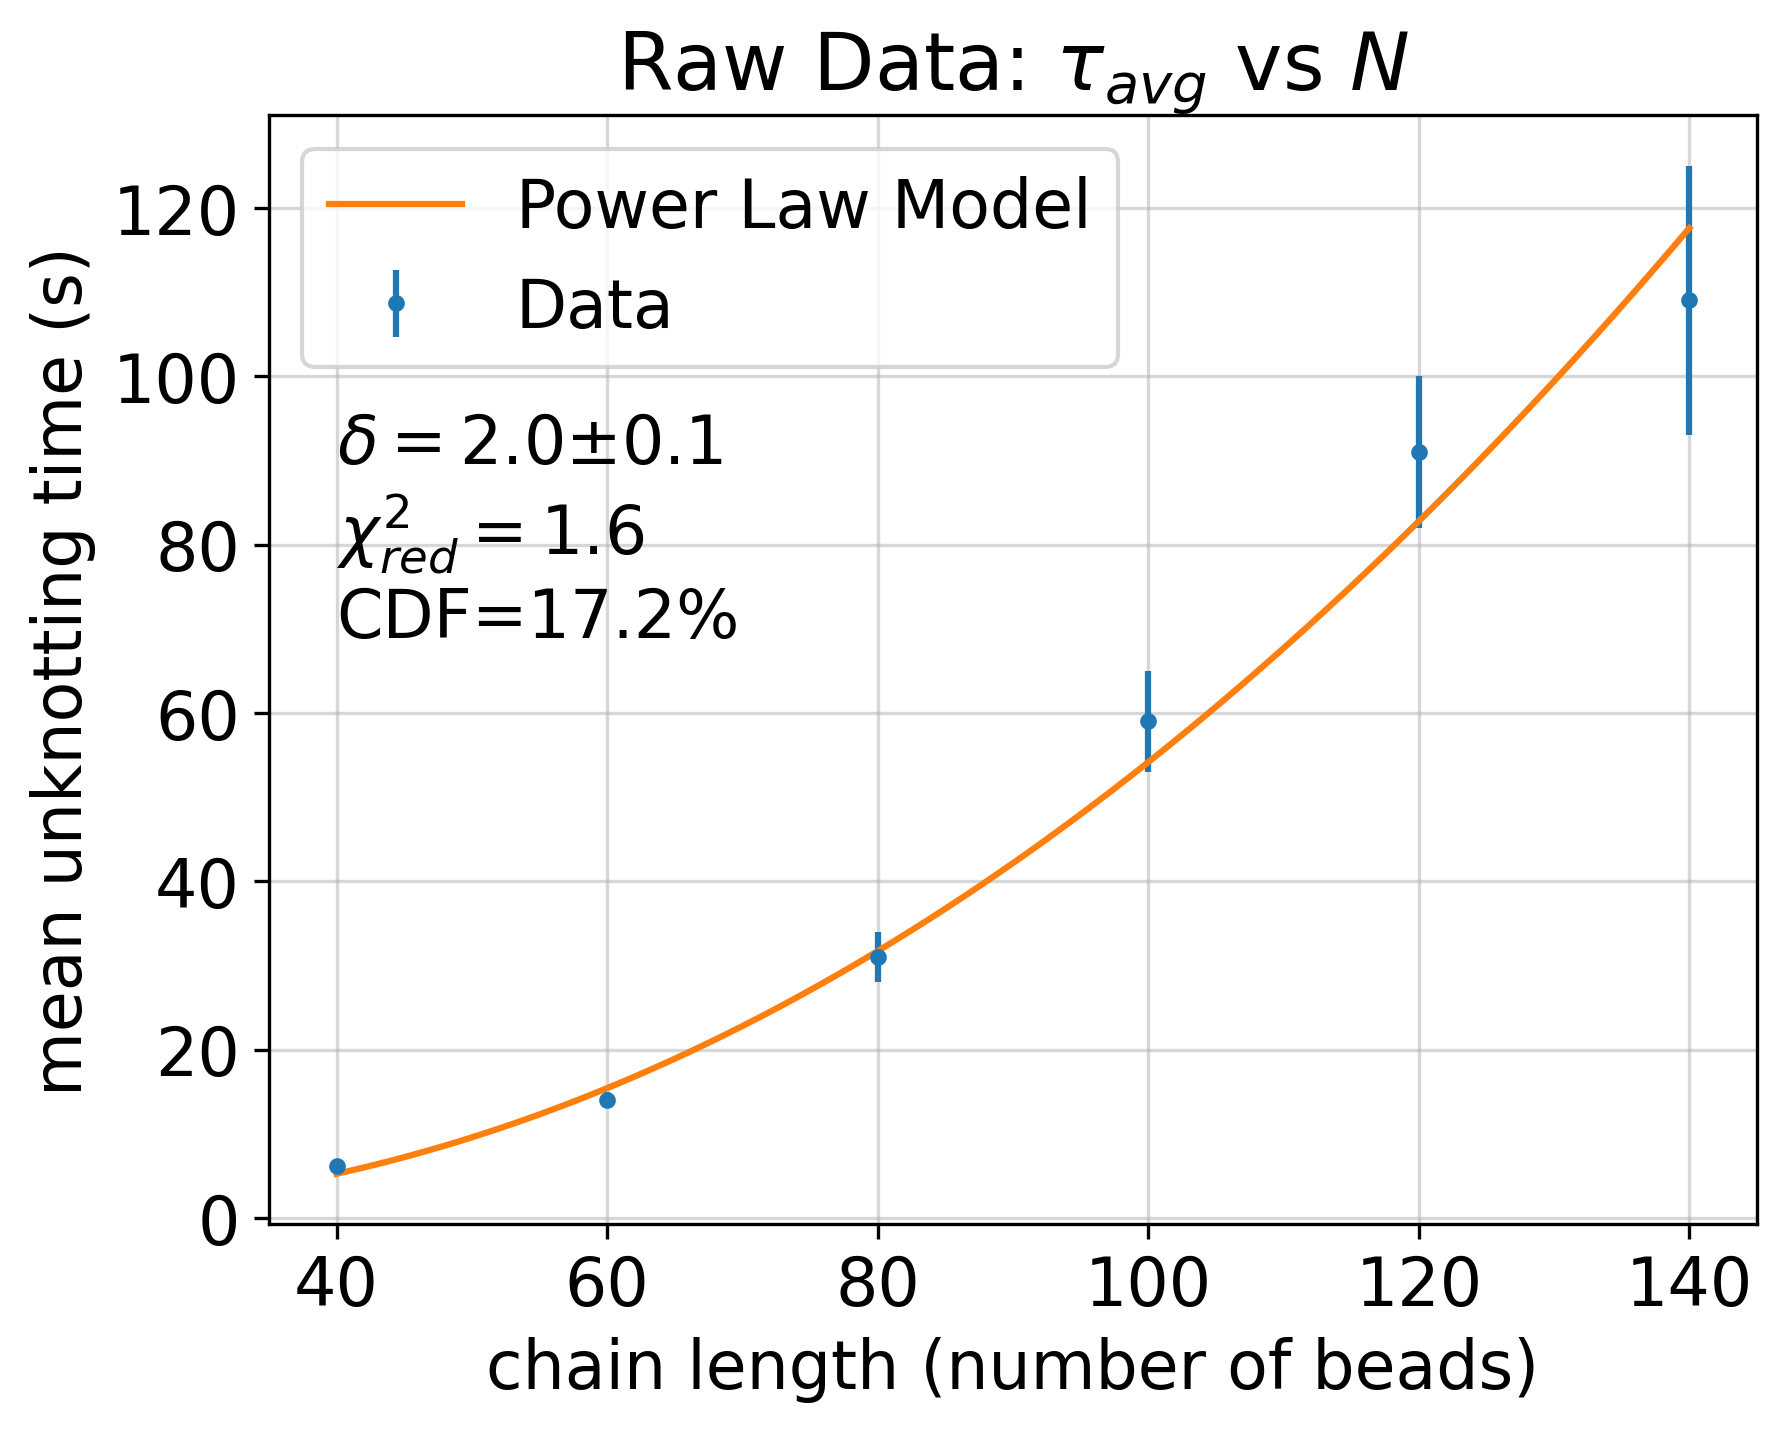
\includegraphics[scale=0.55]{raw.png}
            \caption{A plot of mean unknotting time vs the chain length. In blue is the raw
            data while the orange line is the best fit curve of the form of equation \ref{eq:fit}. 
            The error bars are given by the standard error of the mean time.}
            \label{fig:raw}
        \end{figure}

    To further improve my data, I plotted a histogram for the time distribution for each $N$, 
    with the number of bins given by Sturge's Rule. Figure \ref{fig:hist} contains an example of such a histogram for $N=80$.\\

        \begin{figure}[H]
            \centering
            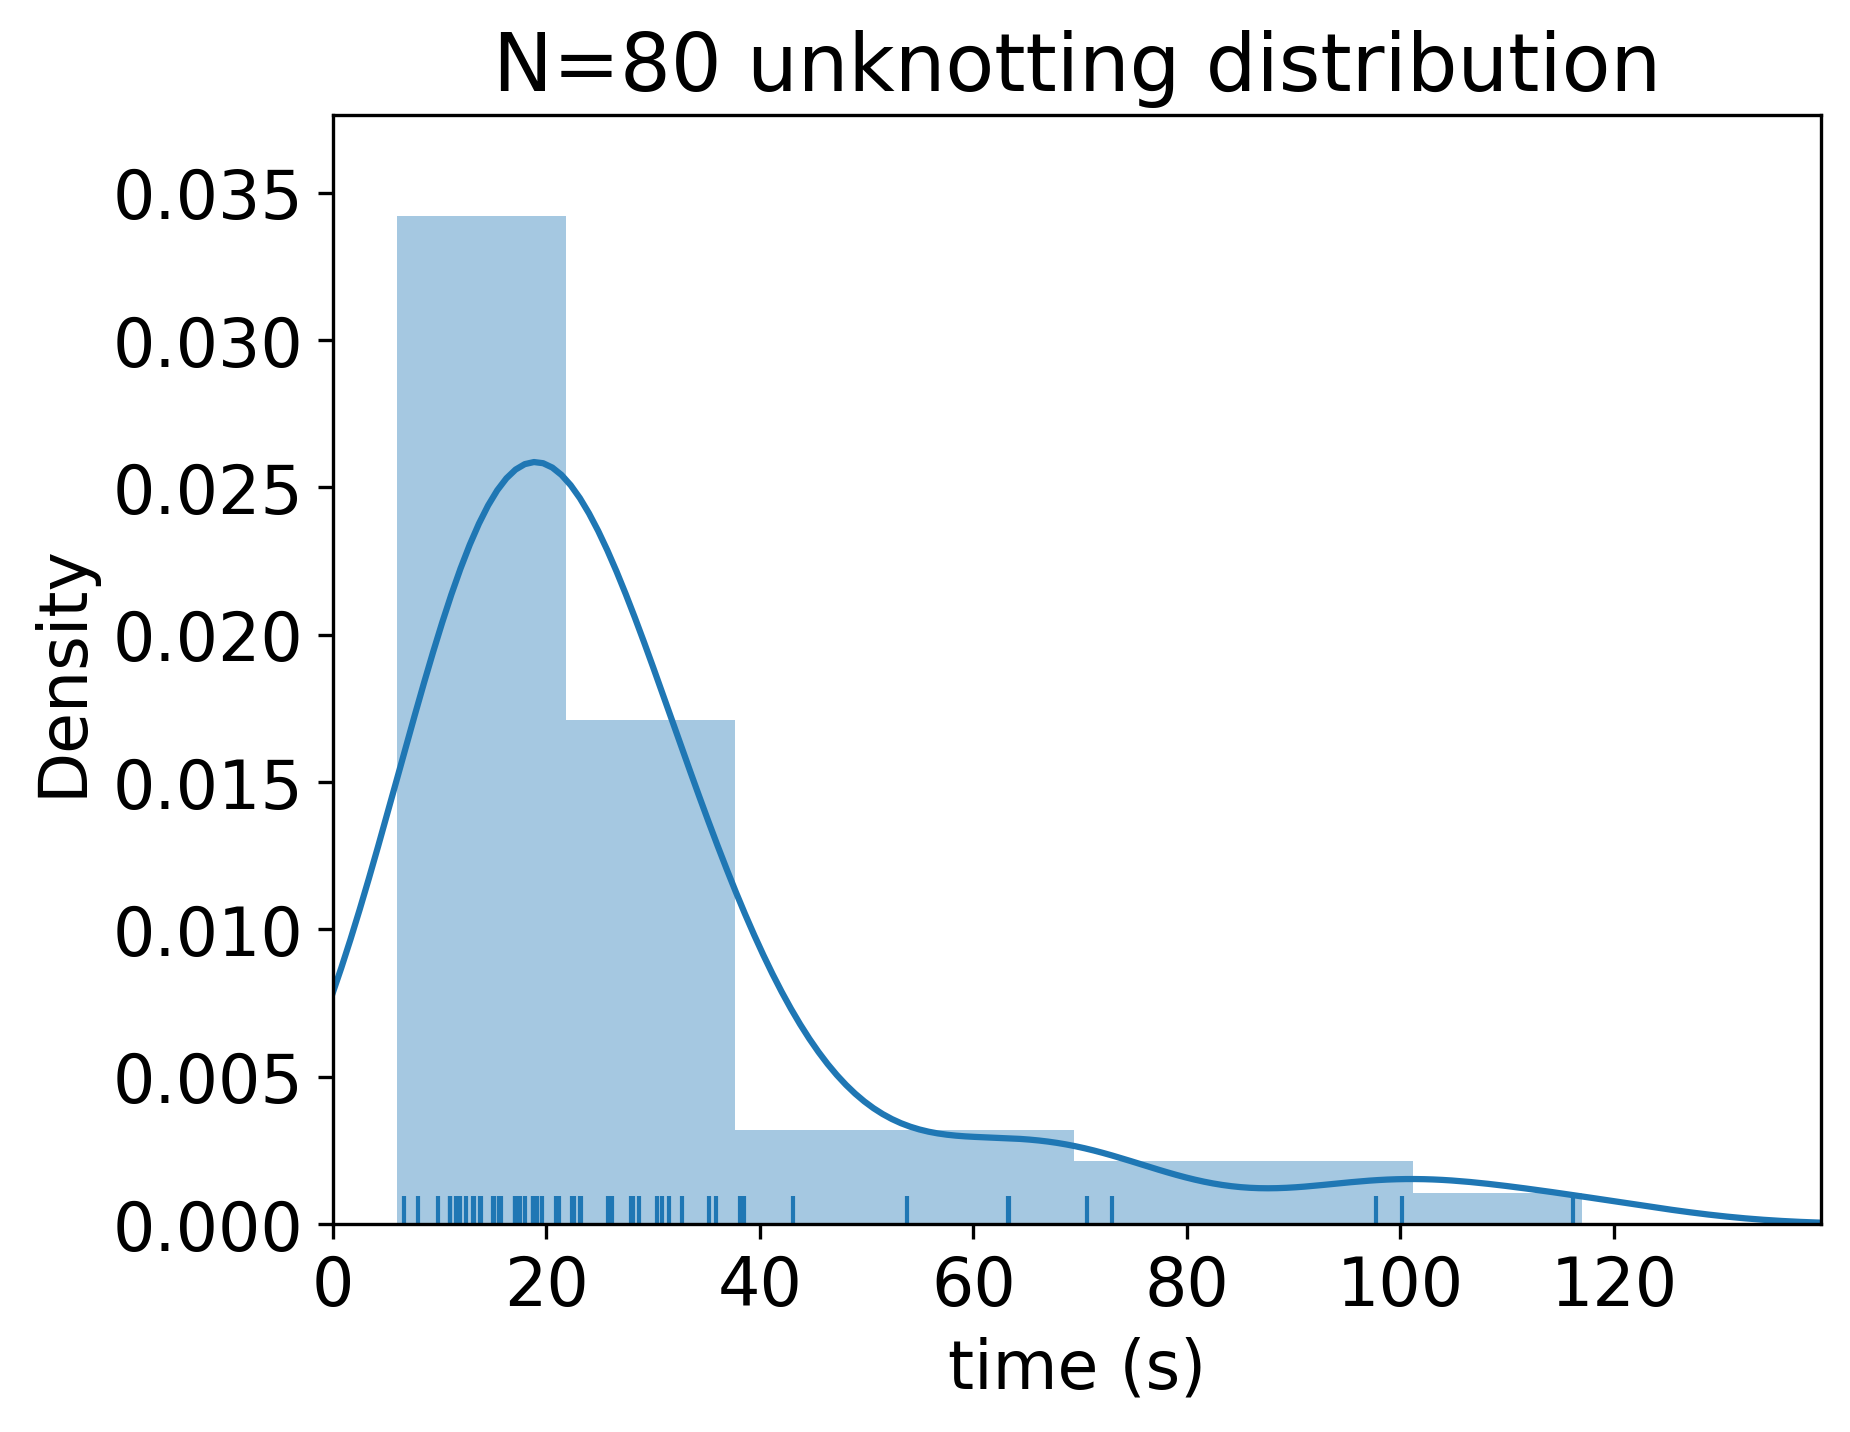
\includegraphics[scale=0.52]{N=80.png}
            \caption{The unknotting time distribution for $N=80$. A kernel density 
            estimate and rug plot is included. Note that the distribution appears Gaussian,
            except for a long tail of anomalously long unknotting times.}
            \label{fig:hist}
        \end{figure}
    I then filtered out the data points in each histogram which were anomalously large. The distribution 
    of unknotting times is not Gaussian due to having a lower bound, but no upper bound. By suppressing
    these high unknotting times, we may get a Gaussian unknotting time distribution and improve the model's results.
    Furthermore, long unknotting times were typically occured in trials where the knot was flipped over or another 
    intersection point was created. Such trials violate the assumptions outlined in Section \ref{sec:theory} and thus 
    cannot be described by the model. The result of fitting the filtered times with equation \ref{eq:fit} is included in Figure 
    \ref{fig:filtered}.
        \begin{figure}[h]
            \centering
            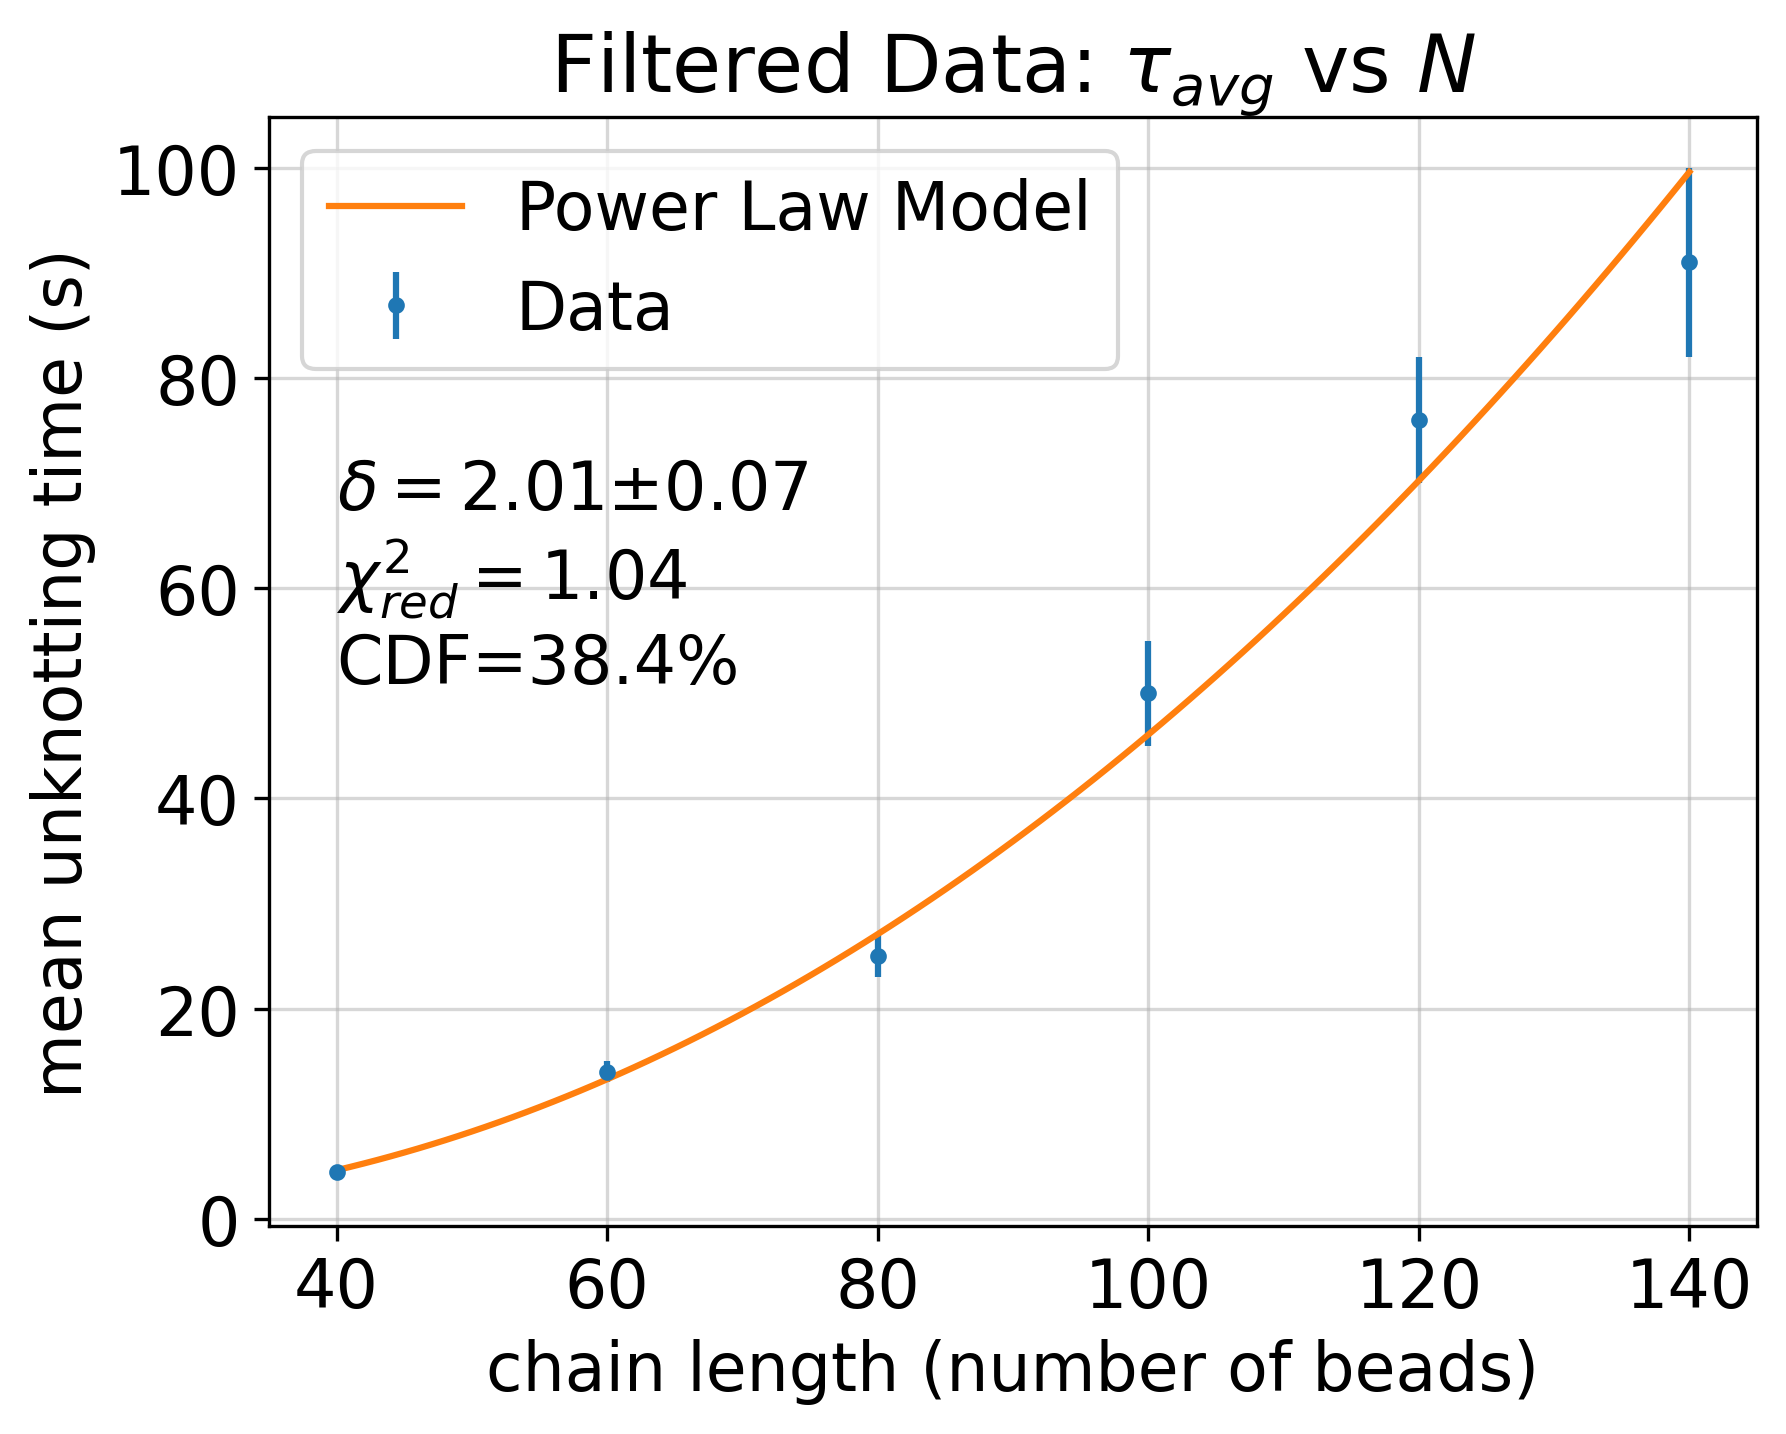
\includegraphics[scale=0.55]{filtered.png}
            \caption{A plot of mean unknotting time vs the chain length. In blue is the filtered
            data while the orange line is the best fit curve of the form of equation \ref{eq:fit}.}
            \label{fig:filtered}
        \end{figure}
    The cdf and reduced chi squared of this new fit indicatees an improvement of the model's ability 
    to describe the behaviour of filtered data, and the resulting best fit parameters were 
    $\delta = 2.01 \pm 0.07$ and diffusivity $D= 9 \pm 3~\unit{s}^{-1}$. 
    Finally, the knot tended to open towards the arm which passed under the loop with overwhelming frequency.
    
    \subsection{Analysis of survival probability}

    Empirically, the survival probability $S(t,N)$ of a knot in a chain of length 
    $N$ at time $t$ can be interpreted as the fraction of unknotting times $\tau$ in a 
    given data set which satisfy $\tau > t$. Plotting this quantity against $t/\tau_\text{avg}$ for each data 
    set results in Figure \ref{fig:survival}.\\
     
        \begin{figure}[h]
            \centering
            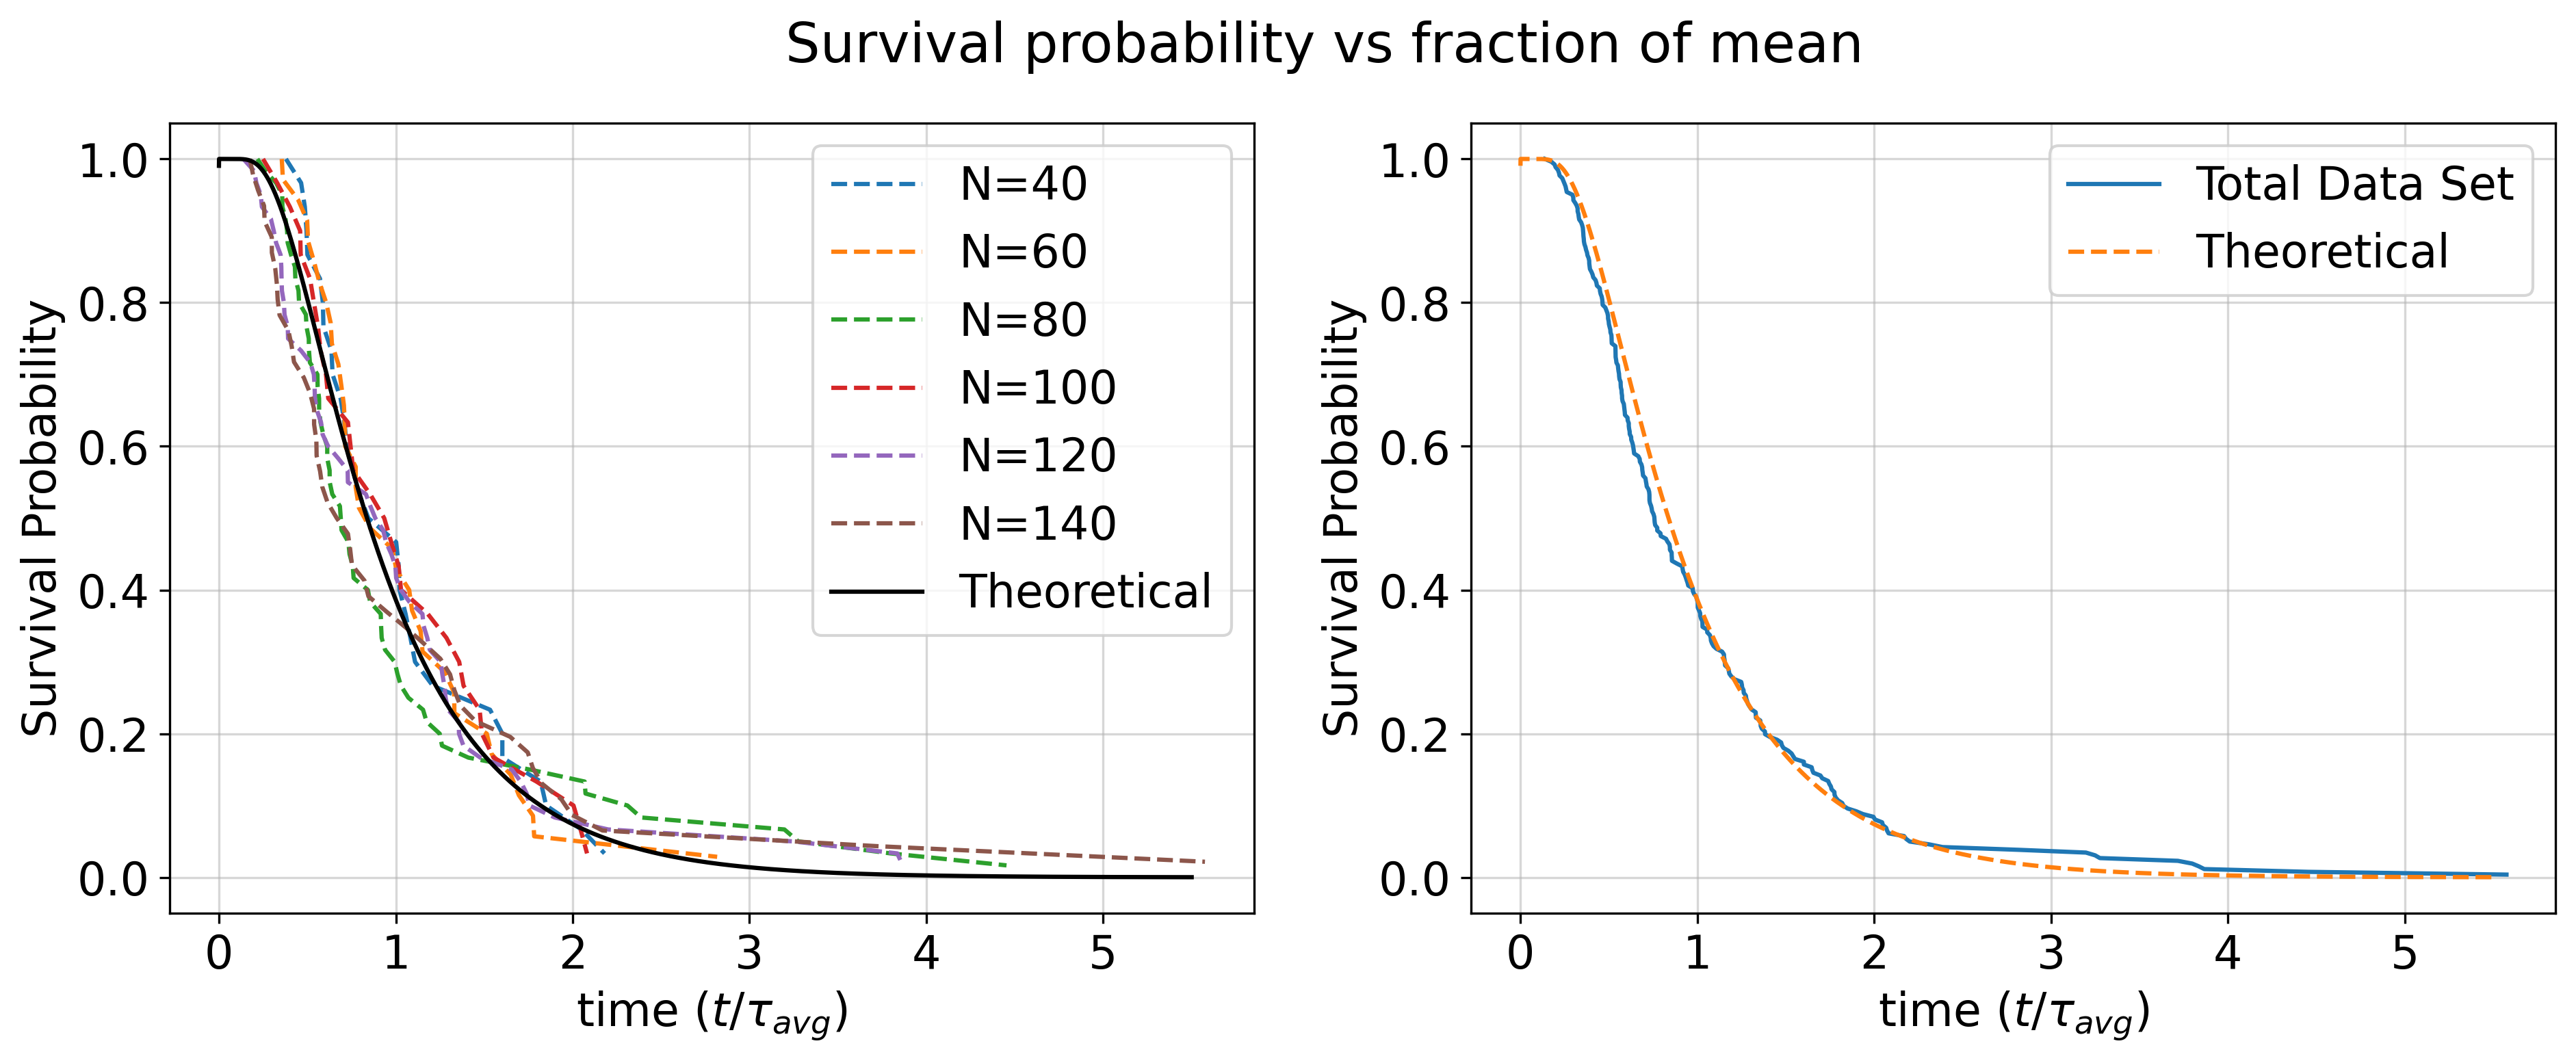
\includegraphics[scale=0.5]{survival.png}
            \caption{Left: The empirical survival probability $S(t,N)$ plotted against
            $t/\tau_\text{avg}$ for each of the six chain length data sets. Right: The empirical
            survival probability plotted against $t/\tau_\text{avg}$ for the conglomeration of each 
            of the six chain length data sets. The theoretical curve is obtained using equation \ref{eq:characteristic}.}
            \label{fig:survival}
        \end{figure}
    
    To find a quanititative measure of the probability that the different survival probability curves 
    come from the same distribution, I used the Komogorov Smirnov test. Given two sample populations, 
    $A$ and $B$, this test returns a p-value for the following null hypothesis: $A$ and $B$ are given by 
    identical distributions. The p-value gives the probability of obtaining the observed results given 
    that the null hypothesis is true.\\

    For each empirical distribution pair, the Komogorov Smirnov test resulted in a p-value of 1.0,
    meaning my data is exactly what one should expect to see if the null hypothesis is true. 
    That is, each survival probability curve is given by the same distirbution.\\

    By performing the Komogorov Smirnov test on the conglomerate data set and a thoeretical data set, 
    obtained from applying $F(z)$ on all the empirically measured exit times, one arrives at a p-value 
    of 0.367, which suggests a 36.7\% chance of obtaining the observed curve if my empirical data set 
    comes from the same distribution as the theoretical data set. 
\section{Conclusions}
    The dynamics of knots in one dimensional filaments are important in determining the macroscopic
    properties of the materials that these filaments comprise. This experiment was successful in 
    studying a simple analog for such system: a trefoil knot in a macroscopic chain.\\

    My final value of $\delta=2.01\pm 0.07$ agrees with equation \ref{eq:mean-exit}. With a reduced 
    chi squared of 1.04 and goodness of fit probability of 38.4\%, I can conclude that Ben-Naim's 
    model accurately predicts the opening times of the trefoil knot as a function of chain length.\\
    
    The diffusivity $D$ can be interpreted as the knot's hopping rate accross the chain. A hopping rate of 
    $D= 9 \pm 3~\unit{s}^{-1}$ is consistent with the oscillation frequency of $f=13$ hz, because there 
    was a significant fraction of oscillations where the chain would not hop over any beads.\\

    When plotted against $z= t/\tau_{\text{avg}}$ as in Figure \ref{fig:survival}, the survival
    probability of the trefoil knot follows the same characteristic curve for each chain length
    $N$. This is evidence in favour of the prediction by \cite{BenNaim2001} that
    \[
        S(t,N) = F(z)
    \]
    In particular, the Komogorov Smirnov test provides strong evidence that the survival probability
    curves for each chain length come from the same distribution, as well as a 36.7\% chance that my data 
    would be obtained if the survival probability is indeed described by $F(z)$. This result is significant 
    because it suggests that the statistics of trefoil knot opening times can be studied independently 
    of the lengths of the chains in which they are embedded, simply by scaling the time scales by the 
    mean exit time for that corresponding chain length. 
\newpage    
\bibliography{references}
\end{document}
